\documentclass[11pt]{article}
\usepackage{amsmath}

\usepackage{graphicx}
\usepackage{enumitem}
\usepackage{placeins}
\usepackage{verbatim}
\usepackage{fancyvrb}
\usepackage{fullpage}
\usepackage{tabularx}
\usepackage{hyperref}

\usepackage{caption}
  \captionsetup{figurename={Figure\ }}
  \DeclareCaptionLabelSeparator{boldperiod}{\textbf{.} }
  \DeclareCaptionFormat{mysmallcaption}{{\footnotesize #1#2#3\par}}
  \DeclareCaptionLabelFormat{bf}{{\rm \bf #1#2}}
  \captionsetup{labelsep=boldperiod,labelformat=bf,format=mysmallcaption}




\setlength{\parskip}{\baselineskip}%
\setlength{\parindent}{0pt}%

\begin{document}

\begin{titlepage}

\begin{center}

\textsc{\LARGE Massachvsetts Institvte of Technology}\\[0.5cm]


% Title
{ \huge \bfseries NARWHAL \\[0.4cm] }
{\Large An Implmentation of Zero Knowledge Authentication}\\[0.5cm]


% Author and supervisor
\begin{minipage}{0.4\textwidth}
\begin{flushleft} \large
\emph{Authors:}\\[0.5cm]
Ryan Cheu \\
{\tt ryancheu@mit.edu} \\[1cm]
Patrick Yang \\
{\tt pbyang@mit.edu} \\[1cm]
Alexander Lin \\
{\tt ajlin@mit.edu} \\[1cm]
Alexander Jaffe \\
{\tt asjaffe@mit.edu}
\end{flushleft}
\end{minipage}
\begin{minipage}{0.4\textwidth}
\begin{flushright} \large

\end{flushright}
\end{minipage}

\vfill

% Bottom of the page
{\large \today}

\end{center}

\end{titlepage}

\section{Abstract}

In this paper, we discuss our implementation of an alternative login system for websites that utilizes a challenge-response model based on zero knowledge proofs.  Our system, called NARWHAL, aims to strengthen a website's authentication system against eavesdropping passive adversaries.  In the course of implementing this system, we have discovered several significant practical shortcomings.  We outline some weaknesses of current login systems, provide a sketch of the protocol (which was originally posed by Lum Jia Jun), discuss implementation issues and tradeoffs, and comment on potential remaining vulnerabilities.

\section{Introduction}

Zero knowledge authentication schemes explore the use of zero knowledge interactive proofs as an alternative model for user authentication.  There are several potential weaknesses of the current canonical model of web authentication, and zero knowledge authentication schemes solve some of these problems cleanly.  We have implemented such a scheme as a system called NARWHAL; our server runs Ruby on Rails and we use JavaScript for client-side computation.

In the course of implementing NARWHAL, we determined that a zero knowledge authentication schems and  most challenge-response authentication schemes could be implemented with little detriment to the user experience.  Still, we also discovered several obstacles that impeded our implementation.  In particular, NARWHAL relies heavily on users having JavaScript enabled in their browsers; even then, we lacked the desired functionality for some cryptographic operations due to a lack of available JavaScript libraries.  In this paper, we outline the system we implemented on both a theoretical and practical level, discussing both advantages and disadvantages of zero knowledge authentication.


\section{Issues with the Current Hashed-Password System}

Most current web authentication solutions use a login form, which sends the username and password to the server as a HTTP request.  In most cases, the password is sent in plain text; sometimes, this plain text password is sent through an SSL connection.  On the server, the password is hashed and compared to a stored hash.  Most systems also use a process called salting in which random bits are added to the end of the password before it is hashed to prevent attacks through pre-computed hash tables\cite{Zhou}.  There are several major attack vectors for this current system.

The first major vector is brute-force hash cracking\cite{Lum}.  In this attack, the adversary has gained access to the hash of the password, usually by compromising the server storing the password hashes.  Once the adversary has access to the password hashes, he hashes many common passwords to see which hash matches and thus determines the original plaintext password.  A user can protect against this attack by choosing a password is difficult to guess, and the server can protect against attacks by choosing a sufficiently secure hashing algorithm and good salts.

A second possible attack is wire sniffing, where a malicious entity listens in on the client's connection to the server and reads the password that's sent over the network\cite{Lum}. Most large sites use SSL for authentication, which encrypts this connection and makes it more difficult for listeniers to read any data; however, some still do not. For example, as of May 2014, the Forbes website (\url{http://www.forbes.com/}) does not log in over HTTPS. If a user were to authenticate with a server over HTTP (not HTTPS) on an unsecured network, such as public Wi-Fi, it would be trivial for an attacker to gain access to the password by sniffing the completely unencrypted packets being sent on the network. 

Additionally, several high-profile password thefts in recent years have occurred when servers stored passwords insecurely (in particular, in plain text or hashed without salting) and then been compromised.  This has been the most publicized form of large-scale password leakage.  When a user sends a password in plaintext and the server does not store this password securely, such catastrophic scenarios may occur.  In January 2013, the servers of dating network Cupid Media were compromised, resulting in the theft of a staggering 42 million unencrypted passwords.  \cite{Donohue}

Finally, the server itself could behave maliciously. Since passwords are almost always sent to the server without hashing, the server can see all passwords in plaintext. Since many users use the same passwords to access multiple sites, a malicious server can simply take this password and other identifiable information about a user (like his or her email) and fraudulently access the victim's accounts on a wide variety of services.

In order to ameliorate these threats, we propose a randomized authentication system based on zero knowledge proofs. This will prevent any information that can be used to easily recover the password from ever be transmitted; furthermore, each login attempt will be different, resulting in a system that is, overall, more secure.

\section{Zero Knowledge Proofs and Applications to Authentication}

Canonical interactive proof systems involve two parties: a Verifier and a Prover\cite{Goldwasser}.  A Verifier presents an instance of a problem to a Prover, and the Prover must provide a verifiable solution. Zero knowledge proofs are a variant on this model, where the Prover provides evidence for the solution's existence without giving away any information about the solution that the Verifier would be unable to compute quickly.  Inherently, zero knowledge proofs are probabilistic: in most zero knowledge proof systems, the Prover can only provide a certificate that demonstrates that he is likely to know the solution; the Verifier obtains confidence through repeated iterations.

This difference between zero knowledge proofs and traditional interactive proofs mirrors the difference between zero knowledge authentication and current login systems.  A zero knowledge authentication scheme would encode the user's identity (e.g. username and password) as a hard problem, and use an interactive zero knowledge proof model to authenticate.

A server running a zero knowledge web authentication system would therefore provide additional resilience against an adversary listening in on server-client messages\cite{Goldwasser}, as this communication cannot be easily exploited to extract sensitive information. Furthermore, the probabilistic nature of zero knowledge proofs is not an issue; in particular, even current client-authentication schemes are not perfectly error-free, as the adversary can simply get lucky and guess the right password by chance.

\section{Original Protocol}
The protocol for zero knowledge authentication that our implementation is based on was described by Lum Jia Jun\cite{Lum}.  We briefly discuss it here to establish notation and correctness. 

\subsection{Setup}

When the server first loads the authentication system, it generates a public key for itself.  This consists of a cryptographic group $G$ as well as some element $g_0$ of $G$\cite{Lum}.

\subsection{Registration}

\begin{figure}[h]
  \centering
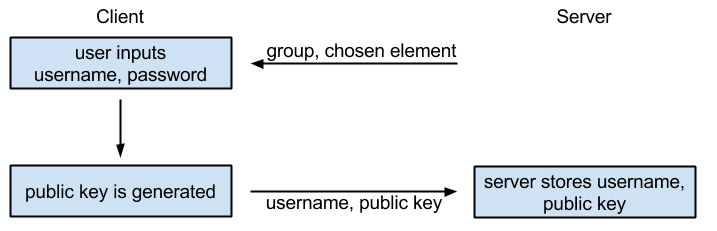
\includegraphics[scale=0.65]{currentauth.png}

 \caption{Registration procedure.}
 \label{fig:registration}
\end{figure}

When a user registers by entering a username and password, the client obtains the server's public key.  Let the hash of the password be $x$; the client computes $Y = g_0 ^ x$ and sends the pair (username, $Y$) to the server.  In particular, the server does not receive the password during registration, and assuming the difficulty of the discrete logarithm problem in $G$, does not receive useful information in determining $x$.  We will refer to $Y$ as the user's public key.\cite{Lum}


\subsection{Authentication}
\begin{figure}[h]
  \centering
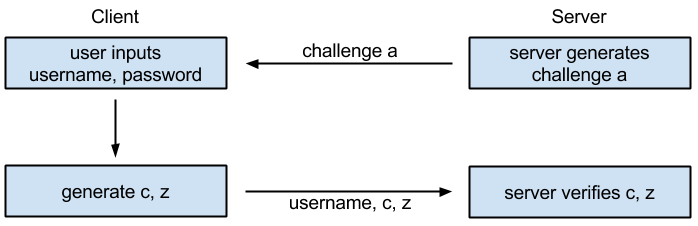
\includegraphics[scale=0.65]{auth.png}

 \caption{Authentication Procedure.}
 \label{fig:authentication}
\end{figure}

To authenticate, the server first generates, stores, and sends the user a challenge in the form of a random number a.  The user then inputs a username and password, and the client calculates the following values:
\begin{itemize}
  \item {\em x} = $hash(password)$
  \item {\em Y} = $g_0 ^ x$
  \item {\em r}, a private random number specific to this authentication attempt
  \item {\em T} = $g_0 ^ r$
  \item {\em c} = $hash(Y || T || a)$
  \item {\em z} = $r - cx$
\end{itemize}
The client then sends the pair (c, z) to the server; we call this pair the user's response.


To confirm the user's identity, the server only needs to confirm the computation of $c$.  Since the server knows both $Y$ and $a$, the server can compute $T' = Y^cg_0^z$.  If $hash(Y || T' || a)$ matches the value of $c$ provided by the user, the server accepts the authentication attempt.\cite{Lum}

\subsection{Correctness}

For a correctly entered password, $T' Y^cg_0z = g_0^{xc + r - cx} = g_0^r = T$, and the server's value of $Y$ will match the value computed by the user.  Thus, the two values of $c$ will also match and the server will always authenticate correctly if given valid credentials.  Refer to Lum Jia Jun's original paper for a more in-depth discussion of correctness and security.


\section{Advantages}

Earlier, we discussed some of the problems with the current login systems.  In this section we'll discuss how our system provides solutions to these problems.

The first issue with traditional login systems occurs when the database is compromised. If passwords are insecurely stored in this database, NARWHAL fares much better; the public keys stored by NARWHAL are intrinsically hard to invert and less vulnerable to rainbow tables. If passwords are securely hashed and salted, NARWHAL makes brute forcing the password from the information stored on the server linearly harder. In a benchmarking test, we used C++ with OpenSSL to compute SHA256 hashes and GMP to compute modular exponentiation on large numbers.  Adding the modular exponentiation requirement increased the running time by a factor of 8. The source code for the test can be found at \url{https://gist.github.com/ryancheu/d2e9fa0432c885e0526c}.  Part of this slowdown is due to the use of numbers larger than 64 bits, meaning that we had to use big number libraries to compute the modular exponentiation.

Another vulnerability of the classical scheme is replay attacks, where an eavesdropper captures valid authentication credentials over a network and replays them to the server at a later time to gain access. Zero knowledge authentication, however, is not susceptible to such attacks.  The login process is randomized, so intercepted credentials are only valid once and in turn do not allow an eavesdropper access with further login attempts.  The information sent to login is also not useful to an adversary without significant computing power.  This means that a password cannot be discovered by intercepting user verification; in contrast, many sites currently send login information in plain text.

Finally, a user can verify that their information is stored securely, since the server never gains direct access to the user's password in the first place.  Right now, the user has no way to know that the server they're authenticating with is not storing their password insecurely or copying it for malicious uses.  With zero knowledge authentication, however, the user can verify that their password is never sent in a readable form and thus ascertain that their password is not being stored or misused.

\section{Our Implementation}

We implemented a website running NARWHAL. Our server is written in Ruby on Rails and sits on a sqlite3 database; the client-side processing is done in JavaScript. Our repository lives at \url{http://github.com/xanderlin/narwhal}.

Upon installation, NARWHAL selects a random prime number of at least 512 bits.  Since the best known general discrete logarithm algorithms are $O(|G|^{1/2})$, where $|G|$ is the size of a group $G$, this number provides 256 bits of entropy.\cite{Adleman}  NARWHAL uses the multiplicative group modulo this prime as its cryptographic group.

\subsection{Registration}

When the user registers, the \texttt{generatePublicKey} JavaScript function hashes the password and generates a public key from the user's password, the user's username, the website's public unique identifier. Each of these three components serves a different function:
\begin{itemize}
  \item the password adds secrecy, as the other two are public information
  \item the username prevents two users of a single website from sharing the same public key
  \item the website's identifier prevents two users with the same username and password on two different websites from sharing the same public key.
\end{itemize}

The client then sends the username and the public key to the server, which stores it into its database and logs the user in.

Unfortunately, we are still unable to salt our public keys with an additional random string. This is further discussed in the ``Potential Remaining Vulnerabilities'' section.

\subsection{Logging In}

When the user goes to a login page, the server provides the client with a random challenge. The client runs the \texttt{addCandZToForm} function to calculate the response, and then sends the username and response to the server. The server verifies these using the stored public key and the random challenge.

The random challenge here is stored in a user's session tokens. These session tokens are bound to a single session; the same user logging in from two different computers will therefore have different session tokens. The ID of a session token (which is a random value corresponding to a single session) is stored in a cookie; when a web request is made, the server looks at this ID to retrieve the other information in a session token.

Currently, random challenges do not expire with time; instead, the session token stores only the most recent random challenge. Every authentication - successful or not - resets this challenge, preventing malicious users from brute forcing a valid response to a randomized challenge.

\subsection{Other Features of Note}

Another feature we considered but did not implement is rate limiting; that is, if multiple failed login attempts on a single user occur, we would ``lock'' a user's account and prevent it from being accessed for a short period of time. We decided that this was a negligible risk because the randomized nature of the challenges would keep the requisite number of iterations to brute force a password very high. In particular, on a website with limited computation power like ours, any attempt to brute force a user's password by repeatedly attempting authorization would result in our server crashing from high traffic flow.

Furthermore, although our implementation is secure from replay attacks, it is still vulnerable to session hijacking if the website is not using HTTPS. This type of attack occurs when a malicious user steals the session ID from a legitimate user and uses sets it in his own cookie to impersonate the victim. HTTPS prevents this by encrypting the connection, making it harder for a user listening to the network to sniff out the session ID.

\section{Implementation Issues}
NARWHAL requires some form of client-side processing. We had numerous options for this; notably, these included applets and trusted third party devices or websites. We ultimately implemented NARWHAL using JavaScript for client side computation, but other options provided unique potential benefits. A brief summary of each of our options for client-side computation follows:

\small
\begin{center}
    \begin{tabular}{|  p{6cm} | p{5cm} | p{5cm} |}
    \hline
    Technology & Pros & Cons \\ \hline
    \vspace{.4cm}
    \textbf{Javascript}
    Each website could have JavaScript, which automatically processes the challenge, username, and password to produce a response. & 

    \begin{itemize}[leftmargin=*]
    \item  Seamless integration and best user experience

    \item  Supported by all modern browsers
    \end{itemize}
    &
    \begin{itemize}[leftmargin=*]
    \item Sometimes disabled for security reasons

    \item Requires more trust in the website
    \end{itemize}
    \\ \hline
    \vspace{.4cm}
    \textbf{Applets}
    This is the approach used by the original paper, which used an applet to download a python script which performed the authentication. We believe this solution is strictly inferior to using JavaScript.
    &
    \begin{itemize}[leftmargin=*]
    \item  Supported by all modern browsers
    \end{itemize}
    &
    \begin{itemize}[leftmargin=*]
    \item Requires a plugin to be installed

    \item Mobile support questionable at best
    \end{itemize}

    \\ \hline
    \vspace{.4cm}
    \textbf{Browser Extention}
    A browser extension could allow the user to easily calculate the response from a challenge, either by manual form entry or by scraping the web page.

    &
    \begin{itemize}[leftmargin=*]
    \item Can easily be verified as secure

    \item Integrates nicely with webpage
    \end{itemize}
    &
    \begin{itemize}[leftmargin=*]
    \item Requires more work by user

    \item Needs to be installed for every browser and computer
    \end{itemize}

    \\ \hline
    \vspace{.4cm}
    \textbf{Client Side Script}
    This is an alternative to a browser extension; the user could download a script or program that they can run to manually calculate the response from the challenge. This would be on either a computer or a phone that the user will have easy access to.

    &
    \begin{itemize}[leftmargin=*]
      \item A downloaded program only needs to be tested once for security.
    \end{itemize}

    &
    
    \begin{itemize}[leftmargin=*]
    \item Requires more work by user
    \item Needs to be installed on a device that can be easily accessed whenever the user wants to log in.
    \end{itemize}        

    \\ \hline
    \vspace{.4cm}
    \textbf{Third Party Website}
    A trusted third party website could function as a service that calculates responses from challenges.
    &

    \begin{itemize}[leftmargin=*]
      \item Portable; easily accessible
    \end{itemize}

    &

    \begin{itemize}[leftmargin=*]
      \item Requires more work by user
      \item If this website gets compromised then a lot of sites get compromised.
    \end{itemize}
    
    \\ \hline
    
    \end{tabular}
\end{center}

\normalsize

We chose JavaScript as it integrates most seamlessly and requires the least work from the user. Javascript, although some users disable JavaScript with applications like NoScript. According to Yahoo in 2010, around $2\%$ of users have JavaScript disabled. \cite{Zakas}

Fortunately, our options for client-side communication are not mutually exclusive; if a user has JavaScript disabled, they can use a trusted third party website and perform the calculation themselves and then manually enter their response to the challenge.

Unfortunately, despite being the option we deemed the most attractive for its simplicity, JavaScript has its own set of difficulties.  In the course of our efforts to implement NARWHAL, we discovered that JavaScript's library support for cryptographic functions is poorly developed, and often even some commonly used libraries proved buggy.  One functionality NARWHAL required in particular was support for large integers.  The large integer library we found and utilized based on recommendations within the JavaScript user community, available online at \url{http://leemon.com/crypto/BigInt.js}, does not support operations on negative numbers.  Such numbers appeared frequently while computing the client's response to the challenge, and forced us to perform inelegant hacks to code ‘around' the library.


\section{Potential Remaining Vulnerabilities}

The protocol as posed by Lum Jia Jun, and as we have implemented, still shares one weakness with a traditional hashed-password protocol where the server does not use salts.  An attacker, targeting a specific server and username, could precompute values of the public key for a list of common passwords, e.g. as a rainbow table.  Then, if the attacker obtained access to the database, he would instantly be able to determine via lookup what the targeted user's password was.  In traditional schemes, salting prevents attacks like this.  However, since the server retains effectively no information about the user's password, the only ways for the client to add a salt in this current protocol are to receive it from the server every time or to store it locally after receiving it at registration time.  Neither modification is appealing: the first is trivially vulnerable to an attacker impersonating the user, and the second relies on the user always having access to the registration device.

Note that this attack doesn't allow the adversary to avoid performing the work of cracking the password.  Rather, it moves the work of discovering a user's password to before the adversary obtains access to the servers.  In this way, a targeted user's account information can be retrieved more rapidly, which potentially lets the attacker access user information before an user is alerted of possible database theft.

However, since these attacks are limited in scope by nature (a separate table must be made for each user) and require massive computation power (with a random 8-character password, there are roughly $2^50$ possible passwords which will take storage space in the exabyte range), we do not expect these attacks to be crippling.

There exist zero knowledge protocols similar to the one used here, but which fix this vulnerability.  For example, the SRP (Secure Remote Password) protocol, developed at Stanford and with existing implementations, solves the issue.  However, the SRP fix comes at the cost of more required computation as well an additional server request. \cite{Wu} 

\section{Conclusion and Future Work}

NARWHAL's simplicity and ease of use for the client demonstrate that, with appropriate setup, a zero knowledge authentication protocol can be feasibly implemented for websites without detriment to the user experience.  Indeed, NARWHAL and other zero knowledge web authentication schemes provide nontrivial benefits, in particular enabling the user to authenticate without ever providing the server with the user's password in plaintext.  However, implementation issues, especially with JavaScript, demonstrated a continued need for improved JavaScript support of cryptographic-related functionality.  Furthermore, NARWHAL more or less requires the user have JavaScript enabled, which forces the user to place some initial trust in the website.

The next step for our work with NARWHAL is to package the system as a Rails gem, enabling easy reuse and distribution.  Other future work includes investigating the existing libraries for JavaScript cryptography and big numbers for correctness, integrity, and security of cryptographic functions, and possibly updating them to meet the needs of NARWHAL should further deficiencies be found.  Also, we could implement one of the protocols that secures against the targeted attack described above, integrating it into NARWHAL. These weaknesses aside, NARWHAL still stands as an effective proof of concept of the zero knowledge authentication concept.

\begin{thebibliography}{9}
\bibitem{Adleman}
Adleman, Leonard M. ``The function field sieve.'' Algorithmic number theory (1994): 108-121.

\bibitem{Donohue}
Donohue, Brian. ``Cupid Media Spills Database of 42 Million Passwords.'' Threatpost. Threatpost, 20 Nov. 2013. Web. 13 May 2014.

\bibitem{Goldwasser}
Goldwasser, Shafi, Silvio Micali, and Charles Rackoff. ``The knowledge complexity of interactive proof systems.'' SIAM Journal on computing 18.1 (1989): 186-208.

\bibitem{Lum}
Lum Jia Jun, Brandon. ``Implementing zero-knowledge authentication with zero knowledge,'' in The Python Papers Monograph 2.9 (2010).

\bibitem{Wu}
Wu, Thomas D. ``The Secure Remote Password Protocol.''NDSS Mar. 1998: 97-111.

\bibitem{Zakas}
Zakas, Nicholas. ``How many users have Javascript disabled?'' Yahoo. Yahoo, 13 Oct. 2010. Web. 13 May 2014.

\bibitem{Zhou}
Zhou, Minqi et al. ``Services in the cloud computing era: A survey.'' Universal Communication Symposium (IUCS), 2010 4th International 18 Oct. 2010: 40-46.

\end{thebibliography}

\end{document}
